\begin{frame}[t]{Regular Type Expressions (RTEs)}

  
  \only<1,2,3>{  We'd like to recognize sequences with  \Emph{regular patterns}.

  \medskip

  {\LARGE [ {1}, \quad
      {2/3},\quad
      {9.3},\quad
      {3},\quad
      {1.5},\quad
      {6.5},\quad
      {4.8},\quad
      {2},\quad
      {2/3}]}
  }%

  \only<2,3>{

  \bigskip

    {\LARGE What's the pattern?}  }%

  \only<3>{{\Large [ \textcolor{greeny}{$\overbrace{1}^{integer}$}
    \textcolor{blue}{$\underbrace{2/3~~ 9.3}_{\text{real}}$}
    \quad \textcolor{greeny}{$\overbrace{3}^{integer}$}
    \textcolor{blue}{$\underbrace{1.5~~ 6.5~~ 4.8}_{\text{real}}$}
    \quad \textcolor{greeny}{$\overbrace{2}^{integer}$}
    \textcolor{blue}{$\underbrace{2/3}_{\text{real}}$}]}
  }%    


  \bigskip

  \only<4,5>{%
  \Large [ \textcolor{greeny}{$\overbrace{1}^{integer}$}
    \textcolor{blue}{$\underbrace{2/3~~ 9.3}_{\text{real}}$}
    \quad \textcolor{greeny}{$\overbrace{3}^{integer}$}
    \textcolor{blue}{$\underbrace{1.5~~ 6.5~~ 4.8}_{\text{real}}$}
    \quad \textcolor{greeny}{$\overbrace{2}^{integer}$}
    \textcolor{blue}{$\underbrace{2/3}_{\text{real}}$}]


  \begin{columns}
    \begin{column}{0.5\textwidth}
          $($
          \textcolor{greeny}{Long}
          $\cdot~ ($
          \textcolor{blue}{Ratio}
          $\cup$
          \textcolor{blue}{Double}
          $) {}^{+} )^{*}$
    \end{column}%
    \begin{column}{0.5\textwidth}
      \only<4>{\scalebox{0.7}{% Modeled after the following
% A simple Tree
% Author: Stefan Kottwitz
% https://www.packtpub.com/hardware-and-creative/latex-cookbook
\documentclass[border=10pt]{standalone}
\usepackage{tikz}
\begin{document}
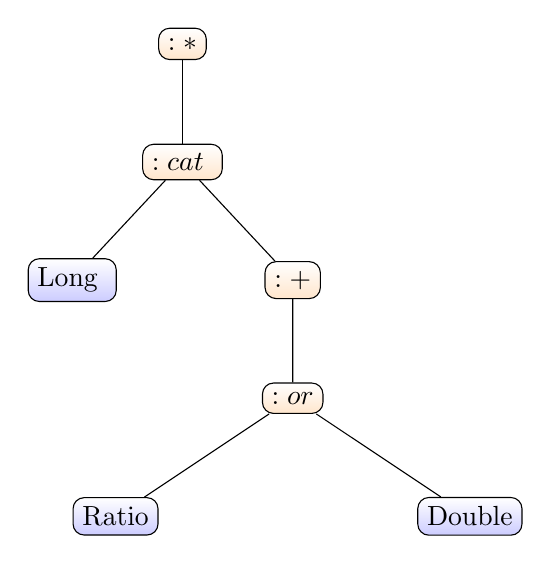
\begin{tikzpicture}[sibling distance=10em,
  every node/.style = {shape=rectangle, rounded corners,
    draw, align=center,
    top color=white, bottom color=orange!20}]]
    \tikzstyle{level 2}=[sibling distance=28mm]
    \tikzstyle{level 4}=[sibling distance=45mm]
  \node {$:*$}
  child { node { $:cat$ } 
    child { node [bottom color=blue!20] {\text{Long} }}
    child { node {$:+$} 
      child { node {$:or$}
        child { node [bottom color=blue!20] {\text{Ratio}} }
        child { node [bottom color=blue!20] {\text{Double}} } } } } ;
\end{tikzpicture}
\end{document}
}}%
      \only<5>{\scalebox{0.7}{\input{strex-clojure-satisfies}}}%
    \end{column}
  \end{columns}
  }
\end{frame}



% use this box via:    \usebox\exnotebox
\newsavebox\exnotebox
\begin{lrbox}{\exnotebox}
  \begin{minipage}{8.5cm}
    %% dont re-indent this file
\begin{lstlisting}[style=conjClojure]
(:* (:cat (satisfies int?)
          (:+ (:or (satisfies float?)
                   (satisfies rational?)))))
\end{lstlisting}

  \end{minipage}
\end{lrbox}

\newsavebox\exnoteexpand
\begin{lrbox}{\exnoteexpand}
  \begin{minipage}{8.5cm}
    %% dont re-indent this file
\begin{lstlisting}[style=conjClojure]
(:* (:cat (:or Long Integer Short Byte)
          (:+ (:or (:or Double Float)
                   clojure.lang.Ratio))))
\end{lstlisting}

  \end{minipage}
\end{lrbox}

\newsavebox\excoreint
\begin{lrbox}{\excoreint}
  \begin{minipage}{7cm}
    %% dont re-indent this file
\begin{lstlisting}[style=conjClojure,numbers=none]
(defn int? [x]
  (or (instance? Long x)
      (instance? Integer x)
      (instance? Short x)
      (instance? Byte x)))
\end{lstlisting}

  \end{minipage}
\end{lrbox}






\begin{frame}{RTEs}{Surface Syntax and AST}
  \begin{columns}
    \begin{column}{0.55\textwidth}
  \begin{itemize}
  \item Mathematical notation:\\
  \quad\textcolor{greeny}{$(Int \cdot (Float \cup Ratio)^+)^*$}
  \item Clojure notation: AST\\
    \usebox\exnotebox
  \item Leaf nodes interface to Clojure/Java Type System
  \end{itemize}
    \end{column}%
    \begin{column}{0.45\textwidth}
      \scalebox{0.8}{\input{strex-clojure-satisfies}}
    \end{column}%
  \end{columns}%
\end{frame}


\begin{frame}{Inlining: thanks \code{clojure.repl.source-fn}}
  \begin{columns}
    \begin{column}{0.6\textwidth}
  \begin{itemize}
  \item Clojure notation: AST\\
    \usebox\exnotebox
  \item Clojure Core\\
    \usebox\excoreint
  \item Inlined\\
    \usebox\exnoteexpand
  \end{itemize}
    \end{column}%
    \begin{column}{0.4\textwidth}
      \scalebox{0.8}{\input{strex-clojure-satisfies}}
    \end{column}%
  \end{columns}
  
\end{frame}

